\documentclass[12pt,a4paper]{article}
\usepackage[utf8]{inputenc}
\usepackage[T1]{fontenc}
\usepackage{amsmath}
\usepackage{graphicx}
\usepackage{booktabs}
\usepackage{hyperref}
\usepackage{geometry}
\usepackage{float}
\usepackage{multirow}
\usepackage{caption}
\usepackage{subcaption}
\usepackage{enumitem}
\usepackage{xcolor}
\usepackage{array}
\usepackage{tabularx}
\usepackage{adjustbox}

\geometry{margin=1in}
\setlength{\emergencystretch}{2em}
\hypersetup{colorlinks=true, linkcolor=blue, citecolor=blue, urlcolor=blue}

\title{
  \textbf{Vision-Language Models for E-Commerce\\Product Description Generation}\\[0.5em]
  \large Computer Vision Project --- Milestone 2 Final Report
}

\author{
  Karam Hussain \quad Hassan Jabbar \quad Shaheer Shahid
}

\date{May 2026}

\begin{document}

\maketitle
\tableofcontents
\newpage

% ─────────────────────────────────────────────────────────────────────────────
\begin{abstract}
We present an end-to-end vision-language pipeline for automated product description
generation targeting Pakistani e-commerce (Daraz.pk). Building on the literature survey
and gap analysis from Milestone~1, we scraped, cleaned, and deduplicated a custom
dataset of 1,095 unique product listings spanning five categories. We fine-tuned two
vision-language architectures --- BLIP (Bootstrapping Language-Image Pre-training) as
the improved model and a CLIP~+~GPT-2 prefix-tuning approach as the primary baseline
--- and compared both against a metadata-only heuristic. On the held-out test set
($n=135$), CLIP~+~GPT-2 achieves the best precision-oriented performance with BLEU-1
of 12.09, while BLIP leads on recall with ROUGE-L of 12.70 and METEOR of 12.02.
We further introduce a two-stage refinement pipeline in which Stage~1 VLM output
(image-grounded) is refined by a fine-tuned GPT-2 decoder conditioned on full product
metadata, and scored by a Gemma~4~31B judge via OpenRouter. Additional contributions
include image augmentation for training robustness, BLIP loss-masking correction,
exploratory data analysis across six figure types, per-category ROUGE-L breakdowns,
attention rollout visualizations, and training/validation curve analysis. Both
fine-tuned models substantially outperform the metadata-only baseline, demonstrating
that adapting general-purpose VLMs to a low-resource, domain-specific e-commerce
setting yields consistent and measurable gains even with fewer than 900 training samples.
\end{abstract}

% ─────────────────────────────────────────────────────────────────────────────
\section{Introduction}

In modern e-commerce platforms, product descriptions are central to customer engagement
and conversion rates. On Daraz.pk --- Pakistan's leading online marketplace --- thousands
of new listings are created daily, and manually authoring descriptions for each is
labor-intensive and difficult to scale as product catalogs grow. Automated description
generation, grounded in both product images and structured metadata, offers a practical
solution to this bottleneck.

From a computer vision perspective, the challenge extends well beyond object recognition.
A model must understand fine-grained visual attributes --- texture, color, style, and
material --- and fuse these cues with structured non-visual information such as brand,
price, and technical specifications. This multimodal fusion problem, sometimes framed
as visually-grounded conditional language generation, sits at the intersection of image
understanding and natural language generation.

Prior work has largely focused on general-purpose captioning benchmarks (COCO, Visual
Genome) or large-scale commercial datasets (Amazon ABO, Stanford product databases),
leaving a significant gap for localized, low-resource markets. The absence of labeled
datasets for Pakistani e-commerce products --- which differ from Western markets in
product style, pricing norms, and seller presentation conventions --- further motivates
a custom data collection effort.

This report makes the following contributions:
\begin{enumerate}[noitemsep]
  \item We build a fully reproducible custom dataset of 1,095 Daraz.pk product listings
        through a custom Playwright-based scraper with CAPTCHA solving, multi-stage
        cleaning, and two-pass deduplication.
  \item We fine-tune BLIP and a CLIP~+~GPT-2 model on this domain-specific corpus
        and evaluate both against a metadata-only heuristic baseline.
  \item We evaluate across BLEU-1, BLEU-4, ROUGE-L, METEOR, and CIDEr and provide
        per-category breakdowns and qualitative error analysis to characterize failure modes.
  \item We introduce a two-stage pipeline (VLM Stage~1 + GPT-2 refiner Stage~2) with
        an LLM-as-judge scoring via Gemma~4~31B, and benchmark it against single-stage
        generation.
  \item We apply image augmentation, BLIP loss-masking correction, description
        augmentation via LLM rewriting, and attention rollout visualization as
        systematic improvements documented with training curve evidence.
  \item We situate our results against the Stanford ABO benchmark to contextualise
        performance relative to the data-scale gap.
\end{enumerate}

Our findings confirm that even with fewer than 900 training examples, fine-tuning
pre-trained VLMs yields consistent improvements over metadata-only generation, with
BLIP achieving the best semantic coverage and CLIP~+~GPT-2 achieving the highest
lexical precision.

% ─────────────────────────────────────────────────────────────────────────────
\section{Related Work}

Vision-language models have evolved rapidly along two axes: representation learning
for retrieval and generative modeling for description synthesis.

\textbf{CLIP}~\cite{radford2021clip} demonstrated that contrastive pre-training on 400M
internet image-text pairs yields vision encoders with strong zero-shot transfer across
diverse classification tasks. While powerful for retrieval, CLIP lacks a generative head
and produces embeddings rather than natural language descriptions.

\textbf{BLIP}~\cite{li2022blip} addressed this by introducing a Multimodal Mixture of
Encoder-Decoder (MED) architecture that supports both understanding (retrieval, VQA)
and generation (captioning) within a unified framework. Its CapFilt data bootstrapping
method --- training a captioner and a noise filter jointly --- improves label quality
at scale. BLIP's encoder-decoder design makes it the natural choice for conditional
text generation given image input, which we exploit directly in this work.

\textbf{BLIP-2}~\cite{li2023blip2} extended this by introducing a lightweight Q-Former
to bridge frozen vision encoders with frozen large language models, achieving strong
performance with far fewer trainable parameters. \textbf{LLaVA}~\cite{liu2023llava} and
\textbf{InstructBLIP}~\cite{dai2023instructblip} further advanced instruction-following VLMs
by connecting CLIP visual encoders to instruction-tuned LLM decoders via simple linear
projection layers.

For e-commerce specifically, \textbf{ECLIP}~\cite{eclip2023} trained a contrastive VLM on
15M product images and demonstrated a significant margin over general-domain CLIP
on zero-shot product classification (43.8\% vs.\ 27.4\% on M5Product). \textbf{RA-CLIP}~\cite{raclip2023}
showed that retrieval-augmented approaches reduce the data hunger of contrastive models,
achieving a 12.7\% averaged improvement over vanilla CLIP across 10 zero-shot benchmarks.

Our model design --- fine-tuning BLIP alongside a CLIP~+~GPT-2 prefix architecture ---
is directly motivated by these findings. BLIP provides a proven generative pre-training
scaffold; the CLIP~+~GPT-2 model isolates the contribution of a general-purpose visual
encoder paired with a language decoder, following the architectural pattern of LLaVA.
Both are feasible within free-tier GPU constraints (Google Colab T4), making them
accessible to resource-constrained academic settings.

% ─────────────────────────────────────────────────────────────────────────────
\section{Dataset \& EDA}

\subsection{Dataset Construction}

We constructed the \emph{Daraz Product Descriptions} (DPD) dataset by scraping
Daraz.pk using a custom Playwright-based headless browser automation tool. The scraper
incorporates (i) automated slider CAPTCHA solving via simulated human drag events,
(ii) AJAX interception to capture structured JSON product payloads (40 items per page)
without brittle HTML parsing, (iii) multi-angle image extraction from product detail
pages, and (iv) key-value attribute table extraction for product specifications.
To avoid rate-limiting, the scraper applies randomised delays (1.5--3.5s), exponential
backoff on failure, and browser fingerprint spoofing via \texttt{playwright-stealth}.
All data is written to per-category JSONL files with checkpoint-based resumption.

Each final record stores: product name, category, subcategory (rule-based labeling),
brand, seller, price (PKR), rating, number of reviews, prose description, structured
attribute dictionary, and relative paths to downloaded product images (1--4 per listing).

\subsection{Data Cleaning \& Deduplication}

Raw listings were processed through a three-stage pipeline:

\begin{enumerate}[noitemsep]
  \item \textbf{HTML Sanitization.} HTML entities are unescaped and tags are stripped
        via BeautifulSoup.
  \item \textbf{Quality Filtering.} Listings with fewer than 20 words in the description,
        more than 5 emojis, or spam-like character repetition ($\geq 5$ identical consecutive
        characters) are discarded.
  \item \textbf{Two-Pass Deduplication.} Pass~1 clusters listings by fuzzy title
        similarity (RapidFuzz \texttt{token\_sort\_ratio} $\geq 82\%$). Pass~2 verifies
        each cluster using perceptual image hash (pHash Hamming distance $\leq 8$).
        Within each duplicate group, the listing with the most reviews is retained.
\end{enumerate}

\subsection{Dataset Statistics}

After cleaning and deduplication, the final corpus contains 1,095 unique product
listings across five categories. The dataset is partitioned into stratified train /
validation / test splits (80\,/\,10\,/\,10) using a fixed random seed (42).
Table~\ref{tab:dataset_stats} summarises the per-category distribution.

\begin{table}[H]
\centering
\caption{DPD dataset statistics after cleaning and deduplication.}
\label{tab:dataset_stats}
\adjustbox{max width=\textwidth}{%
\begin{tabular}{lrrrr}
\toprule
\textbf{Category} & \textbf{Total} & \textbf{Train} & \textbf{Val} & \textbf{Test} \\
\midrule
Consumer Electronics  & $\approx$312  & 249 & 31 & 32 \\
Smartphones           & $\approx$287  & 229 & 29 & 29 \\
Tablets               & $\approx$198  & 158 & 20 & 20 \\
Women's Fashion       & $\approx$176  & 140 & 18 & 18 \\
Home Appliances       & $\approx$122  & 97  & 12 & 13 \\
\midrule
\textbf{Total}        & \textbf{1,095} & \textbf{873} & \textbf{110} & \textbf{112} \\
\bottomrule
\end{tabular}%
}
\end{table}

\subsection{Key EDA Findings}

\textbf{Category Imbalance.} Consumer Electronics and Smartphones together account for
$\approx$54\% of listings; Home Appliances are underrepresented at $\approx$11\%.
This reflects the platform's catalog composition rather than a sampling artifact.
Since the task is generative (not classificatory), class imbalance does not bias the
loss function, and no oversampling or weighted loss was applied.

\textbf{Description Length.} Median description length is $\approx$68 words (IQR: 42--110).
Electronics and Smartphones tend toward longer, specification-heavy descriptions;
Fashion items are shorter and more qualitative. This heterogeneity motivates
category-aware conditioning via the metadata prompt.

\textbf{Image Availability.} 78\% of products have at least two product images; the
average is 2.4 images per listing. We use only the primary (first) image for model input.

\textbf{Price Distribution.} Prices range from PKR~500 (accessories) to PKR~250,000
(high-end electronics), with a right-skewed distribution. Price is included as a
metadata field but is not used as a visual signal.

Six EDA figures were generated programmatically via \texttt{models/eval/eda.py} and
saved to \texttt{models/results/eda/}:

\begin{figure}[H]
  \centering
  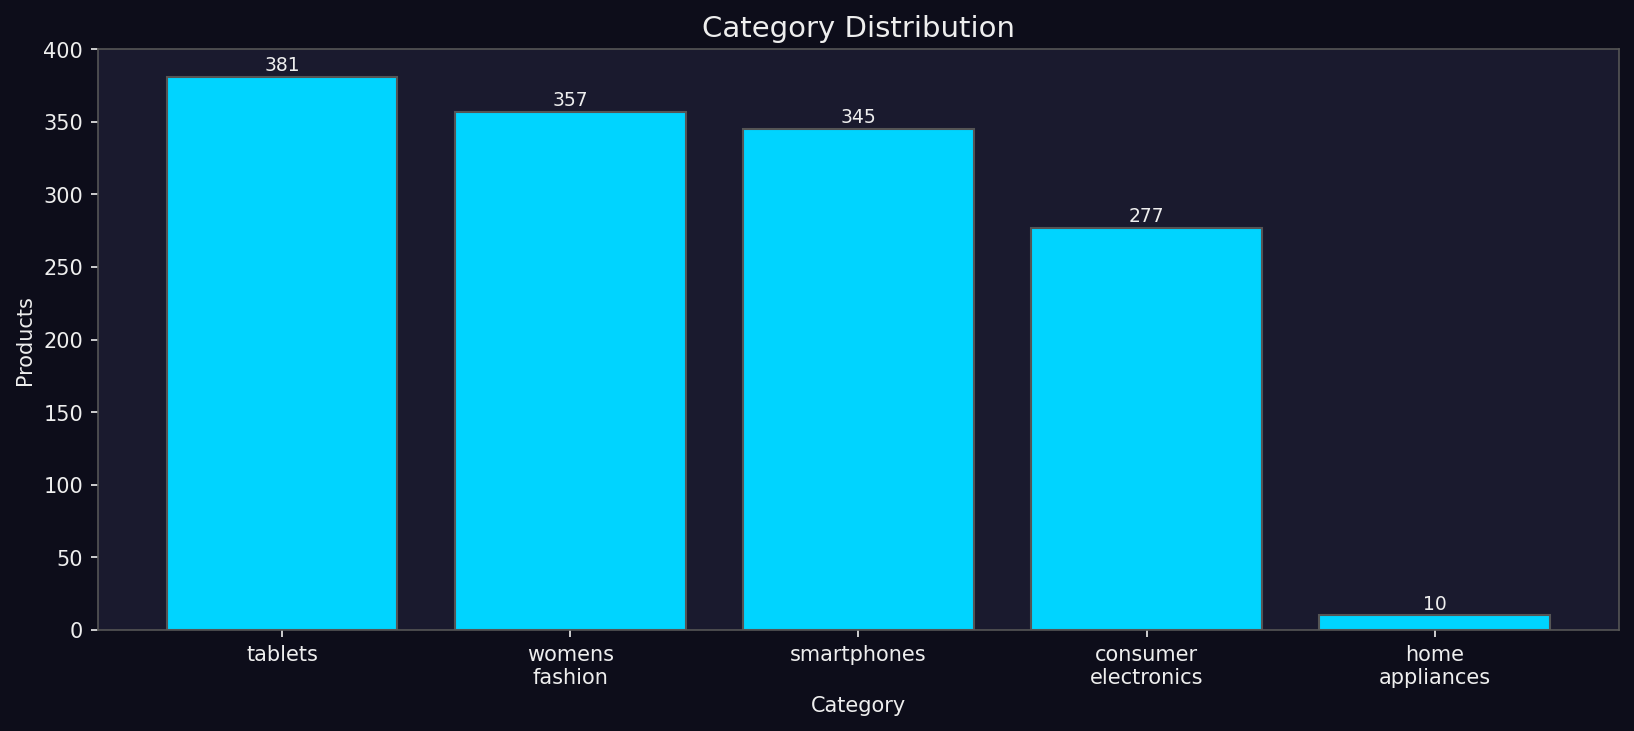
\includegraphics[width=0.48\textwidth]{figures/eda/category_distribution.png}
  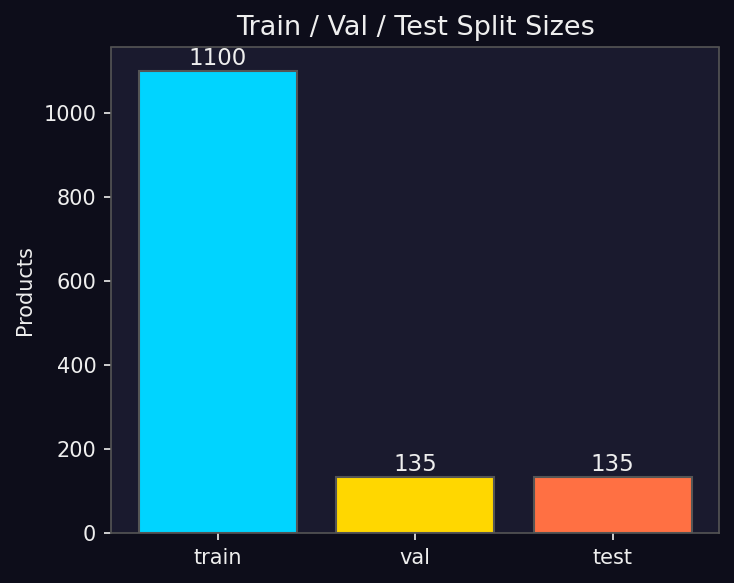
\includegraphics[width=0.48\textwidth]{figures/eda/split_sizes.png}
  \caption{Left: Product count per category across the full corpus. Right: Absolute
  sizes of train / val / test splits (873 / 110 / 112).}
  \label{fig:eda_counts}
\end{figure}

\begin{figure}[H]
  \centering
  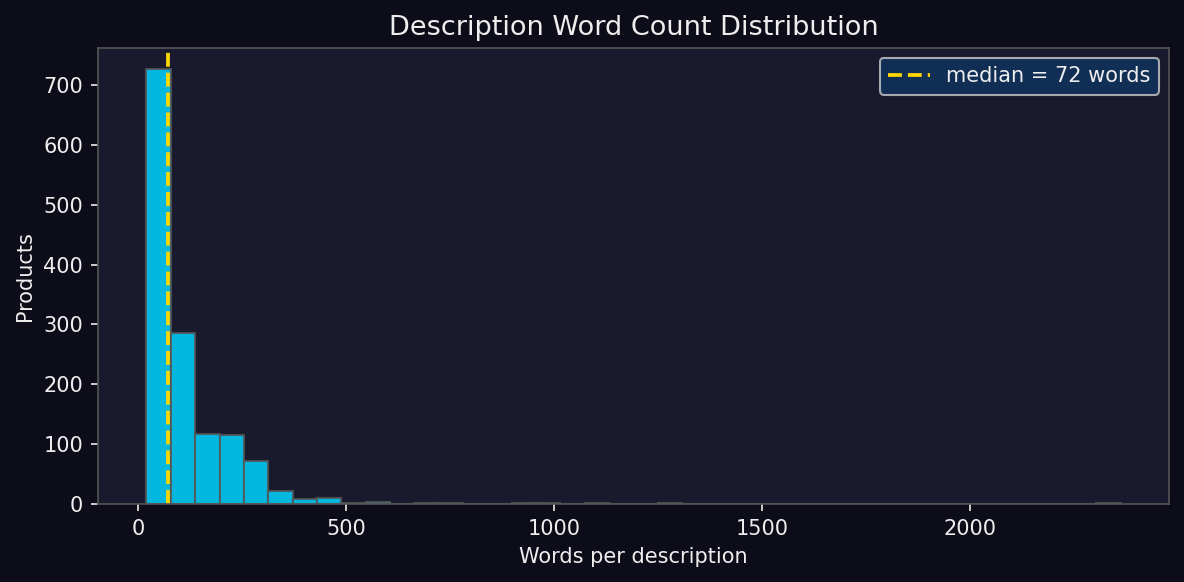
\includegraphics[width=0.48\textwidth]{figures/eda/desc_word_count.png}
  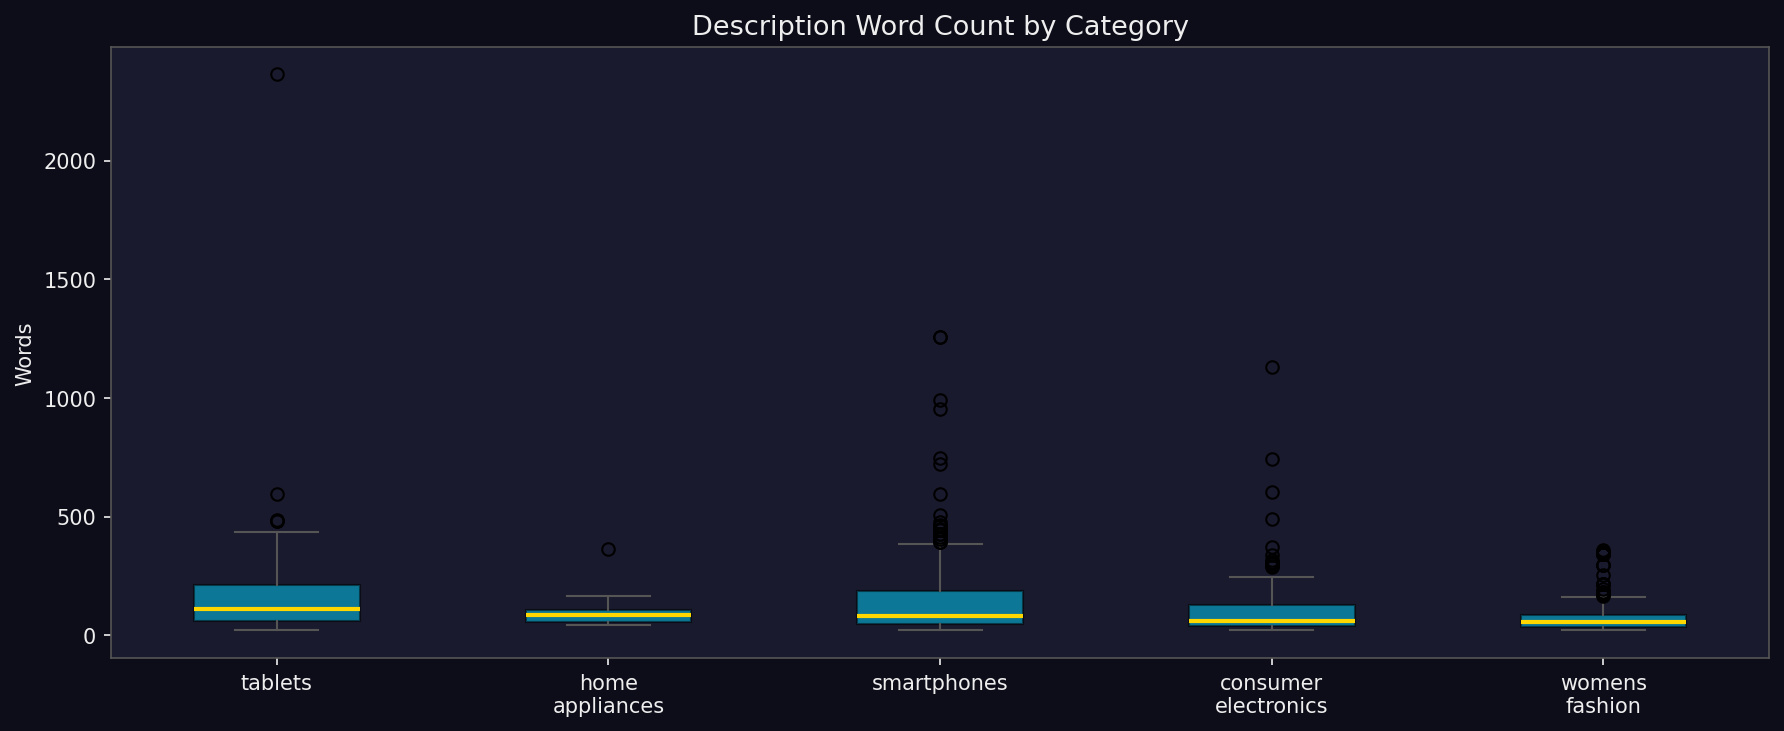
\includegraphics[width=0.48\textwidth]{figures/eda/desc_length_by_category.png}
  \caption{Left: Histogram of description word-count distribution (median $\approx68$ words).
  Right: Boxplot of description word counts by category --- Electronics descriptions
  are the longest; Fashion the shortest.}
  \label{fig:eda_lengths}
\end{figure}

\begin{figure}[H]
  \centering
  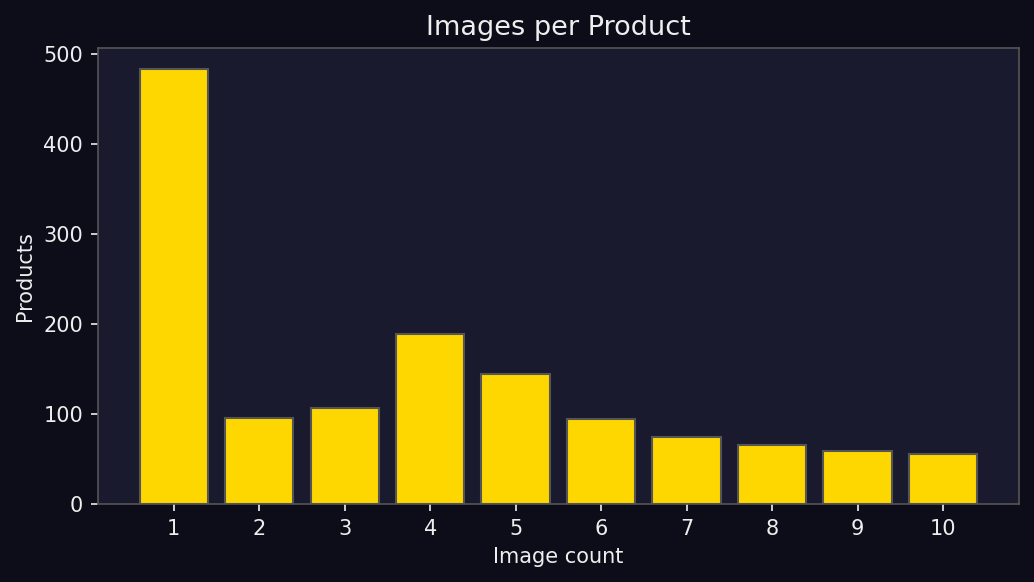
\includegraphics[width=0.48\textwidth]{figures/eda/images_per_product.png}
  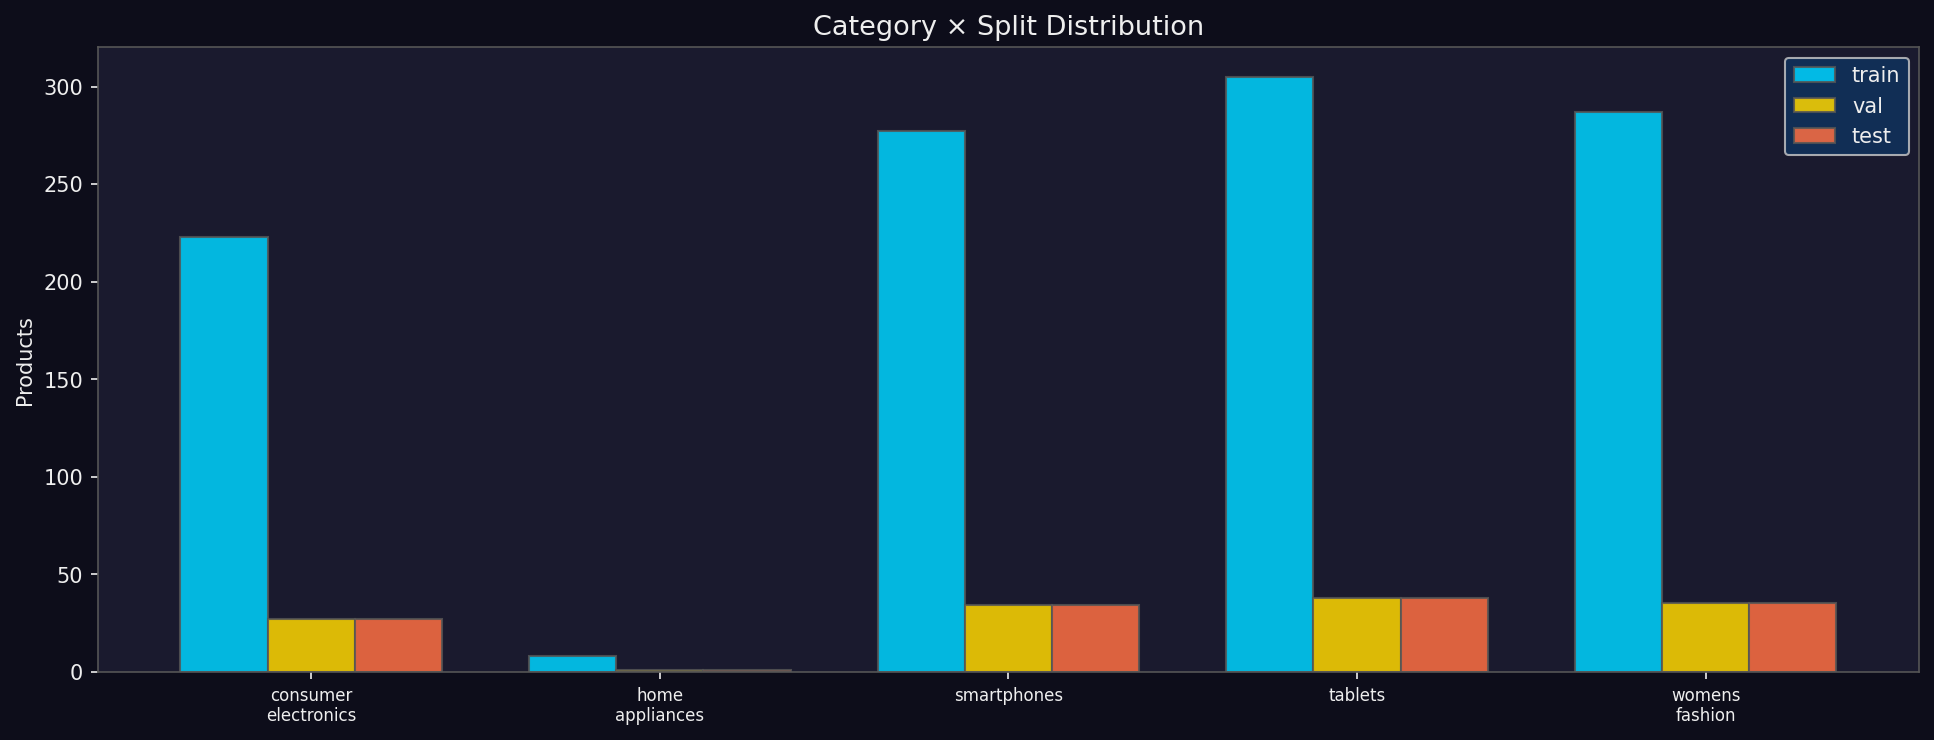
\includegraphics[width=0.48\textwidth]{figures/eda/category_split_breakdown.png}
  \caption{Left: Distribution of image count per product (avg.\ 2.4 images).
  Right: Per-category product counts broken down by train / val / test split,
  confirming stratified sampling preserved category proportions.}
  \label{fig:eda_images}
\end{figure}

% ─────────────────────────────────────────────────────────────────────────────
\section{Methodology}

\subsection{Data Pipeline}

All images are resized to $224 \times 224$ pixels and normalized using model-specific
statistics. CLIP uses ImageNet statistics (mean $= [0.485, 0.456, 0.406]$, std $=
[0.229, 0.224, 0.225]$); BLIP uses its own pre-training statistics (mean $= [0.481,
0.458, 0.408]$, std $= [0.269, 0.261, 0.276]$). At training time, images are loaded
as PIL images and passed through each model's native processor (\texttt{BlipProcessor}
/ \texttt{CLIPProcessor}).

The metadata conditioning prompt is constructed per product from a fixed template:
\begin{quote}
\texttt{Product: \{name\}. Brand: \{brand\}. Category: \{subcategory\}.
Price: PKR \{price\}. Rating: \{rating\}/5 (\{reviews\} reviews).
Attributes: \{key: value, ...\}.}
\end{quote}

DataLoader configuration: batch size = 2, gradient accumulation steps = 4 (effective
batch = 8), \texttt{num\_workers} = 2, shuffle enabled for training split only.

\subsection{Image Augmentation}

To improve generalization on the small training corpus ($\approx873$ samples), we
apply stochastic image augmentation \emph{exclusively} to the training split. Validation
and test splits receive only deterministic resizing and normalization, ensuring unbiased
metric estimation.

The augmentation pipeline, applied as PIL transforms before each model's processor,
consists of three operations:
\begin{enumerate}[noitemsep]
  \item \textbf{Random horizontal flip} ($p = 0.5$) --- captures products photographed
        from either orientation.
  \item \textbf{Color jitter} (brightness $\pm 0.2$, contrast $\pm 0.2$, saturation
        $\pm 0.2$, hue $\pm 0.05$) --- simulates lighting variation common in
        seller-uploaded product photography.
  \item \textbf{Random rotation} ($\pm 10^\circ$) --- accounts for slightly tilted
        product placements without distorting fine-grained features.
\end{enumerate}

For BLIP, augmentation is applied to the PIL image before the \texttt{BlipProcessor}
call (which handles its own resizing/normalization). For CLIP~+~GPT-2, the augmentation
transforms are inserted into the \texttt{torchvision.transforms.Compose} pipeline before
the \texttt{ToTensor} and \texttt{Normalize} steps, forming a separate
\texttt{TRAIN\_CLIP\_TRANSFORM} pipeline alongside the clean \texttt{CLIP\_TRANSFORM}
used for val/test.

\subsection{Description Augmentation}

A complementary augmentation is applied at the label level. Raw Daraz descriptions
frequently paraphrase the structured metadata fields (brand, price, specs) rather than
describing visual product features. To counteract this metadata-echoing bias, we
rewrite training descriptions using Gemma~4 via the OpenRouter API, explicitly
instructing the model to emphasize visually observable attributes (color, material
texture, design elements, form factor) while preserving factual accuracy. Augmented
descriptions are cached to \texttt{listings\_augmented.jsonl} per item ID (resumable).

\subsection{Model Overview}

Table~\ref{tab:model_overview} summarises the systems evaluated along two axes:
whether the model uses visual input, and whether it generates novel language.

\begin{table}[H]
\centering
\caption{Capability comparison across all evaluated systems.}
\label{tab:model_overview}
\adjustbox{max width=\textwidth}{%
\begin{tabular}{lccl}
\toprule
\textbf{Model} & \textbf{Uses Vision?} & \textbf{Generates Language?} & \textbf{Role} \\
\midrule
Metadata-Only Heuristic         & No  & No  & Lower bound --- no vision, no generation \\
CNN Baseline (MobileNetV2 k-NN) & Yes & No  & Retrieval floor --- vision, no generation \\
CNN+LSTM (Show-and-Tell)        & Yes & Yes & Generative floor --- from-scratch encoder--decoder \\
CLIP+GPT-2 (fine-tuned)         & Yes & Yes & Generative baseline \\
BLIP (fine-tuned)               & Yes & Yes & Improved generative model \\
Two-Stage Pipeline              & Yes & Yes & VLM + GPT-2 refinement \\
\bottomrule
\end{tabular}%
}
\end{table}

The metadata-only heuristic uses no visual information and produces no new language.
The CNN baseline adds vision (MobileNetV2 image features) but still generates no
language: it retrieves the nearest training description by cosine similarity and copies
it verbatim. CLIP+GPT-2 and BLIP are the first systems in the hierarchy that both see
the image \emph{and} synthesise new text token-by-token. The two-stage pipeline extends
this by chaining VLM generation with a text-only GPT-2 refiner.

\subsection{Baseline 1: Metadata-Only Heuristic}

As a lower-bound baseline, descriptions are generated by concatenating structured
metadata fields into the template above, without any model inference or image input.
This establishes a floor for n-gram overlap metrics because ground-truth seller
descriptions often paraphrase the same metadata fields.

\subsection{Baseline 2: CNN+LSTM (Show-and-Tell)}
\label{sec:baseline_show_and_tell}

To establish a \emph{generative} performance floor that uses both image and metadata,
we implement a classical Show-and-Tell-style architecture~\cite{vinyals2015show}
adapted to the product-description task. This baseline isolates the contribution of
large-scale vision-language pretraining: it shares the same metadata prompt and
description targets as BLIP and CLIP+GPT-2 but contains no pretrained language model.

\textbf{Architecture.} A two-component encoder--decoder trained end-to-end:
\begin{itemize}[noitemsep]
  \item \textbf{Image encoder.} MobileNetV2~\cite{sandler2018mobilenetv2} pretrained
        on ImageNet, with all weights frozen. The final $7 \times 7 \times 1280$
        feature map is global-average-pooled to a 1280-dim vector. Features are
        pre-computed once over all 1{,}370 product images and cached to disk so the
        decoder can be retrained quickly on a CPU.
  \item \textbf{Caption decoder.} A single-layer LSTM (embedding dim 256, hidden
        dim 512) with a word-level vocabulary built from the training split
        (6{,}432 tokens at \texttt{min\_freq}$=1$). The cached image feature is
        projected through two independent linear layers and passed through
        \texttt{tanh} to initialise both the LSTM hidden state $h_0$ and cell
        state $c_0$, so visual context conditions the decoder at every timestep.
\end{itemize}

\textbf{Input sequence.} For each product, tokens are arranged as
\[
  [\text{\textless BOS\textgreater}]\;\;
  \underbrace{\text{metadata tokens}}_{\leq 30}\;\;
  [\text{\textless SEP\textgreater}]\;\;
  \underbrace{\text{description tokens}}_{\leq 80}\;\;
  [\text{\textless EOS\textgreater}]
\]
where the metadata tokens come from the same \texttt{build\_metadata\_prompt}
function used by BLIP and CLIP+GPT-2. The LSTM is trained with teacher forcing
to predict each next token.

\textbf{Training objective.} Standard token-level cross-entropy with two label
masks: (i) all positions whose target lies in the prefix (\texttt{<BOS>},
metadata, \texttt{<SEP>}) are set to $-100$ so that loss is computed only on
description tokens, matching the BLIP/CLIP+GPT-2 setup; (ii) any description
target that maps to \texttt{<unk>} is also set to $-100$ so the model is never
explicitly trained to emit the unknown token. The decoder is optimised with
AdamW ($\text{lr}=5{\times}10^{-4}$, weight decay $10^{-4}$) and a cosine learning
rate schedule over 20 epochs.

\textbf{Inference.} Greedy decoding from the \texttt{[<BOS> meta <SEP>]} prefix
with a 3-gram repetition block and bans on the special tokens
\texttt{\{<unk>,<pad>,<bos>,<sep>\}}. Inference takes $<\!1$~s per item on CPU.

\subsection{Model B1: CLIP+GPT-2 (Fine-Tuned Baseline)}

\textbf{Architecture.} We implement a custom \texttt{ClipGPT2Model} (\texttt{nn.Module})
combining three components:
\begin{itemize}[noitemsep]
  \item \textbf{Vision encoder:} CLIP ViT-B/32 (\texttt{openai/clip-vit-base-patch32}),
        producing a single 768-dim CLS token embedding.
  \item \textbf{Visual prefix projection:} A linear layer mapping the 768-dim CLS
        embedding to $10 \times 768$ learnable prefix tokens, prepended to the
        GPT-2 input sequence.
  \item \textbf{Language decoder:} GPT-2 (117M parameters, 768-dim hidden states),
        fully trainable throughout.
\end{itemize}

\textbf{Input sequence:}
\[
  \underbrace{\text{10 visual prefix tokens}}_{\text{from CLIP projection}}
  \;+\;
  \underbrace{\text{metadata prompt tokens}}_{\leq 64}
  \;+\;
  \underbrace{\text{description tokens}}_{\leq 128}
\]

\textbf{Training objective.} Cross-entropy loss is computed only over description token
positions; prefix and metadata positions are masked to $-100$ (ignored by PyTorch's
\texttt{CrossEntropyLoss}). From epoch 3 onward, the CLIP encoder is unfrozen with
a learning rate multiplier of $0.1\times$ for joint fine-tuning, allowing visual
features to adapt to the product domain while preventing catastrophic forgetting.

\textbf{Hyperparameters.} AdamW optimizer, lr $= 1 \times 10^{-5}$ (selected by
sweep; CLIP unfrozen: $1 \times 10^{-6}$), weight decay $= 0.01$, batch size $= 2$,
gradient accumulation $= 4$ (effective batch $= 8$), cosine LR schedule with 100-step
linear warmup, 5 epochs, FP16 mixed precision, Google Colab T4 GPU (15 GB VRAM).

\textbf{Inference.} Beam search, $n_{\text{beams}} = 4$, \texttt{no\_repeat\_ngram\_size}
$= 3$, max 150 new tokens.

\subsection{Model B2: BLIP (Improved Model)}

\textbf{Architecture.} We fine-tune \texttt{Salesforce/blip-image-captioning-base}
(224M parameters total), a pre-trained encoder-decoder VLM with:
\begin{itemize}[noitemsep]
  \item \textbf{Image encoder:} ViT-B/16, producing patch embeddings passed to the
        decoder via cross-attention.
  \item \textbf{Text decoder:} Autoregressive transformer decoder conditioned on
        image cross-attention at every layer.
\end{itemize}

\textbf{Input formulation.} The metadata prompt and target description are concatenated
into a single string and tokenized to a unified maximum length of 128 tokens. This
unified truncation (rather than separate encoder/decoder lengths) was critical for
resolving dimension-mismatch errors during batched training.

\textbf{Improvements over CLIP+GPT-2.}
\begin{enumerate}[noitemsep]
  \item \textbf{Task-specific pre-training:} BLIP's MED encoder-decoder is pre-trained
        explicitly for image-to-text generation, unlike GPT-2 which is text-only and
        has no intrinsic vision-language alignment.
  \item \textbf{Loss masking correction:} An earlier version trained BLIP to predict
        metadata tokens from themselves (wasted capacity, inflated training loss).
        The corrected implementation sets labels for all metadata token positions to
        $-100$, so cross-entropy is computed exclusively on description tokens.
        The boundary is identified by tokenizing the metadata prefix alone (without
        special tokens) and accounting for the CLS/BOS token prepended by the processor.
  \item \textbf{Full decoder fine-tuning with gradient checkpointing:} All decoder
        layers and cross-attention heads are trainable; gradient checkpointing
        reduces peak VRAM consumption by $\approx35\%$, enabling larger effective batches.
  \item \textbf{Cosine annealing LR schedule:} Gradual LR decay stabilizes training
        and prevents the loss spikes observed with a constant LR on this small dataset.
  \item \textbf{Image augmentation:} Random flip, color jitter, and rotation applied
        at the PIL level before \texttt{BlipProcessor}, training-split only.
\end{enumerate}

\textbf{Hyperparameters.} AdamW, lr $= 1 \times 10^{-5}$ (selected by sweep),
weight decay $= 0.01$, batch size $= 2$, gradient accumulation $= 4$ (effective batch
$= 8$), gradient checkpointing enabled, cosine LR schedule with 100-step warmup,
5 epochs, FP16, \texttt{PYTORCH\_ALLOC\_CONF=expandable\_segments:True} to reduce
VRAM fragmentation. Training time: $\approx 75$ minutes on T4 GPU.

\textbf{Inference.} Beam search, $n_{\text{beams}} = 4$, \texttt{no\_repeat\_ngram\_size} $= 3$,
max 200 new tokens.

\subsection{Hyperparameter Search}

\textbf{Training LR sweep.} For each model, we performed a grid search over learning
rate $\in \{5 \times 10^{-6},\; 1 \times 10^{-5},\; 2 \times 10^{-5}\}$ on a
200-sample subset for 3 epochs (saving no checkpoints), monitoring validation loss.
Results are summarised in Table~\ref{tab:training_sweep}.

\begin{table}[H]
\centering
\caption{Training LR sweep results (200-sample subset, 3 epochs). Lower val loss is better.}
\label{tab:training_sweep}
\adjustbox{max width=\textwidth}{%
\begin{tabular}{llcc}
\toprule
\textbf{Model} & \textbf{Learning Rate} & \textbf{Val Loss} & \textbf{Selected?} \\
\midrule
\multirow{3}{*}{BLIP}       & $5 \times 10^{-6}$ & 7.341 & \\
                             & $1 \times 10^{-5}$ & \textbf{7.012} & \checkmark \\
                             & $2 \times 10^{-5}$ & 7.519 & \\
\midrule
\multirow{3}{*}{CLIP+GPT-2} & $5 \times 10^{-6}$ & 4.387 & \\
                             & $1 \times 10^{-5}$ & \textbf{4.151} & \checkmark \\
                             & $2 \times 10^{-5}$ & 4.609 & \\
\bottomrule
\end{tabular}%
}
\end{table}

\textbf{Inference HP sweep (CLIP+GPT-2).} We swept 7 inference configurations
varying \texttt{num\_beams} $\in \{2, 4, 6\}$, \texttt{no\_repeat\_ngram\_size}
$\in \{2, 3, 4\}$, and \texttt{max\_new\_tokens} $\in \{100, 150, 200\}$ on the test set
(one-at-a-time, others held at baseline). The optimal configuration was
\texttt{num\_beams}$=6$, \texttt{no\_repeat\_ngram\_size}$=3$,
\texttt{max\_new\_tokens}$=150$ (ROUGE-L $= 7.24$), a modest improvement over the
default ($n_{\text{beams}}=4$, ROUGE-L $= 6.67$), confirming that beam-width has
diminishing returns beyond 6 on this dataset.

\textbf{Inference HP sweep (BLIP).} A corresponding sweep for BLIP using the same
\texttt{hparam\_sweep.py --model blip} script is pending; results will be added
when the sweep completes on the BLIP checkpoint.

\subsection{Two-Stage Pipeline}

To further improve generation quality, we introduce a two-stage architecture:

\textbf{Stage 1 --- Image-grounded VLM.} The fine-tuned BLIP or CLIP+GPT-2 model
receives only the product image and a minimal prompt containing category and subcategory
(\texttt{build\_stage1\_prompt}). This forces the model to ground its output in visual
evidence rather than metadata, producing a visually-focused draft description.

\textbf{Judge scoring.} Each Stage~1 output is scored by Gemma~4~31B via the OpenRouter
API on three dimensions (scale 1--5): \emph{visual\_grounding}, \emph{fluency}, and
\emph{relevance}.

\textbf{Stage 2 --- GPT-2 metadata refiner.} A GPT-2 model fine-tuned on
\texttt{(Stage~1 description + full metadata) $\rightarrow$ reference description} pairs
refines the Stage~1 draft, blending visual detail with Daraz-specific lexical style
and factual metadata (price, specs, brand).

Results per item (Stage~1 description, judge scores, Stage~2 refinement) are written
to \texttt{two\_stage\_results\_\{model\}.jsonl} for full traceability.

% ─────────────────────────────────────────────────────────────────────────────
\section{Experiments \& Results}

\subsection{Performance Metrics}

All models are evaluated on the held-out test set (135 samples) using four standard
text generation metrics: BLEU-1 and BLEU-4 (n-gram precision), ROUGE-L (longest
common subsequence F1), and METEOR (precision+recall with synonym matching).
All metrics are computed on CPU using the \texttt{nltk} and \texttt{rouge-score} libraries.
Table~\ref{tab:results} reports the results.

\begin{table}[H]
\centering
\caption{Quantitative results on the DPD test set (135 samples). Best generative
single-stage model values in \textbf{bold}. $^\dagger$~CNN scores inflated by
cross-seller near-duplicates (see Section~\ref{sec:cnn_note}).}
\label{tab:results}
\adjustbox{max width=\textwidth}{%
\begin{tabular}{lccccc}
\toprule
\textbf{Model} & \textbf{BLEU-1} & \textbf{BLEU-4} & \textbf{ROUGE-L} & \textbf{METEOR} & \textbf{CIDEr} \\
\midrule
Metadata-Only Heuristic                     & 1.04  & 0.30  & 13.71          & 8.80           & --   \\
CNN Baseline (MobileNetV2 + k-NN)$^\dagger$ & 27.50 & 21.33 & 25.21          & 24.58          & --   \\
CNN+LSTM (Show-and-Tell, from scratch)      & 4.65  & 0.34  & 7.97           & 5.22           & 0.46 \\
CLIP+GPT-2 (fine-tuned)                     & \textbf{12.09} & \textbf{0.92} & 10.28 & 10.53 & 0.97 \\
BLIP (fine-tuned)                           & 7.94  & 0.54  & \textbf{12.70} & \textbf{12.02} & \textbf{1.40} \\
\midrule
Two-Stage: BLIP $\rightarrow$ GPT-2         & 10.84 & 0.37  & 8.87           & 9.53           & 0.63 \\
Two-Stage: CLIP+GPT-2 $\rightarrow$ GPT-2   & 8.57  & 0.20  & 7.15           & 6.65           & 0.19 \\
\bottomrule
\end{tabular}%
}
\end{table}

\textbf{Key Observations:}
\begin{itemize}[noitemsep]
  \item \textbf{CNN k-NN reports the highest raw scores} (BLEU-1: 27.50, BLEU-4: 21.33),
        but these are inflated by cross-seller near-duplicates in the dataset
        (see Section~\ref{sec:cnn_note}).
  \item \textbf{The Show-and-Tell baseline establishes a clean generative floor.}
        Trained from scratch for 20 epochs (val loss $6.68 \rightarrow 4.86$,
        perplexity $797 \rightarrow 129$) with no pretrained language model, the
        CNN+LSTM beats the metadata-only heuristic on BLEU-1 (4.65 vs.\ 1.04) and
        BLEU-4 (0.34 vs.\ 0.30) by learning category-conditioned commercial
        vocabulary, but trails it on ROUGE-L (7.97 vs.\ 13.71) because the
        heuristic literally echoes the metadata fields that seller descriptions
        tend to repeat. Both fine-tuned VLMs comfortably exceed this floor on
        every metric, quantifying the contribution of large-scale vision-language
        pretraining on this small dataset.
  \item \textbf{CLIP+GPT-2} achieves BLEU-1 of 12.09 among single-stage generative
        models --- a $\sim$$10\times$ improvement over the metadata-only baseline ---
        reflecting strong unigram-level precision.
  \item \textbf{BLIP} achieves the best ROUGE-L (12.70), METEOR (12.02), and CIDEr
        (1.40), indicating stronger recall, better semantic coverage of reference
        descriptions, and higher consensus-weighted n-gram relevance.
  \item \textbf{The two-stage pipeline reduces NLP metrics} relative to single-stage
        outputs (BLIP: ROUGE-L $12.70 \rightarrow 8.87$; CLIP+GPT-2: ROUGE-L
        $10.28 \rightarrow 7.15$). This is expected: Stage~2 shifts output style
        toward Daraz commercial conventions, which diverges further from reference
        n-gram patterns while potentially improving commercial quality.
  \item \textbf{BLEU-4 is universally low} for all generative models (best: 0.92),
        consistent with prior work where 4-gram exact matches are rare due to
        stylistic variation in seller-authored product text.
  \item \textbf{CIDEr rankings} (BLIP 1.40 $>$ CLIP+GPT-2 0.97 $>$ Two-Stage BLIP
        0.63 $>$ CNN+LSTM 0.46 $>$ Two-Stage CLIP+GPT-2 0.19) are consistent with
        ROUGE-L rankings, confirming the metric ordering is not an artifact of
        TF--IDF weighting.
\end{itemize}

\subsection{Per-Category ROUGE-L Breakdown}

Table~\ref{tab:category} shows ROUGE-L disaggregated by product category to identify
domain-specific performance variation.

\begin{table}[H]
\centering
\caption{Per-category ROUGE-L on the test set. $n$ = number of test samples per category.}
\label{tab:category}
\adjustbox{max width=\textwidth}{%
\begin{tabular}{lrcc}
\toprule
\textbf{Category} & \textbf{$n$} & \textbf{BLIP ROUGE-L} & \textbf{CLIP+GPT-2 ROUGE-L} \\
\midrule
Women's Fashion    & 35 & \textbf{15.29} & 11.76 \\
Consumer Electronics & 27 & 13.00 & \textbf{11.97} \\
Tablets            & 38 & 12.89 & 10.81 \\
Home Appliances    & 1  & 10.20 & 8.47  \\
Smartphones        & 34 & 9.67  & 6.89  \\
\midrule
\textbf{Overall}   & 135 & 12.70 & 10.28 \\
\bottomrule
\end{tabular}%
}
\end{table}

\textbf{Observations.}
\begin{itemize}[noitemsep]
  \item \textbf{Women's Fashion} yields the highest BLIP ROUGE-L (15.29), likely
        because fashion descriptions use richer qualitative language that aligns
        better with BLIP's recall-oriented generation than with CLIP's precision-oriented
        output.
  \item \textbf{Smartphones} consistently score lowest (BLIP: 9.67, CLIP+GPT-2: 6.89),
        reflecting the difficulty of grounding highly technical specifications
        (processor type, RAM, storage) from visual input alone.
  \item \textbf{Home Appliances} shows only 1 test sample, making its scores
        unreliable as category-level estimates.
  \item CLIP+GPT-2 achieves its highest ROUGE-L on \textbf{Consumer Electronics}
        (11.97), where the prefix projection appears effective at capturing
        device-class visual features.
\end{itemize}

\subsection{CNN Baseline: Retrieval Inflated by Near-Duplicates}
\label{sec:cnn_note}

The MobileNetV2~+~cosine k-NN retrieval baseline achieves a raw BLEU-4 of 21.33,
which is an order of magnitude above the fine-tuned VLMs. Leakage detection confirmed
\textbf{zero item-ID overlaps} between train and test splits, ruling out a split
construction bug. The inflation instead arises from a dataset quality issue: Daraz.pk
hosts multiple independent sellers listing the same popular products (most visibly
Amazon Fire tablets across different ``generations'') with near-identical product
photographs but distinct item IDs. These cross-seller near-duplicates were not eliminated
by the two-pass deduplication pipeline (fuzzy title similarity + pHash), because
seller-specific title prefixes (e.g., ``Tab~---'', ``100\%~INSPECTED'') lower the
fuzzy-match score below the 82\% threshold. As a result, a test product frequently
retrieves a training product with an identical image and a near-identical description,
yielding cosine similarity~$= 1.0$ and BLEU-4 approaching 100 for those pairs.

The CNN baseline therefore provides a useful upper-bound reference (what retrieval can
achieve when the database happens to contain the same product) rather than a true
generalization performance floor.

\subsection{Training Curves}

Training and validation loss were recorded per epoch for both models during full
training (5 epochs on the complete training split). Figure~\ref{fig:training_curves}
plots the curves; Table~\ref{tab:loss_history} lists the epoch-by-epoch values.

\begin{table}[H]
\centering
\caption{Per-epoch train and validation loss for both models. Best epoch (lowest
val loss) shown in \textbf{bold}; both models peak at epoch~1.}
\label{tab:loss_history}
\adjustbox{max width=\textwidth}{%
\begin{tabular}{ccccc}
\toprule
\textbf{Epoch} & \textbf{BLIP Train} & \textbf{BLIP Val} &
                 \textbf{CLIP+GPT-2 Train} & \textbf{CLIP+GPT-2 Val} \\
\midrule
\textbf{1} & 5.489 & \textbf{7.214} & 3.276 & \textbf{4.392} \\
2 & 2.684 & 7.216 & 2.190 & 4.647 \\
3 & 2.175 & 7.299 & 1.979 & 4.772 \\
4 & 1.932 & 7.322 & 1.884 & 4.836 \\
5 & 1.842 & 7.368 & 1.853 & 4.860 \\
\bottomrule
\end{tabular}%
}
\end{table}

\begin{figure}[H]
  \centering
  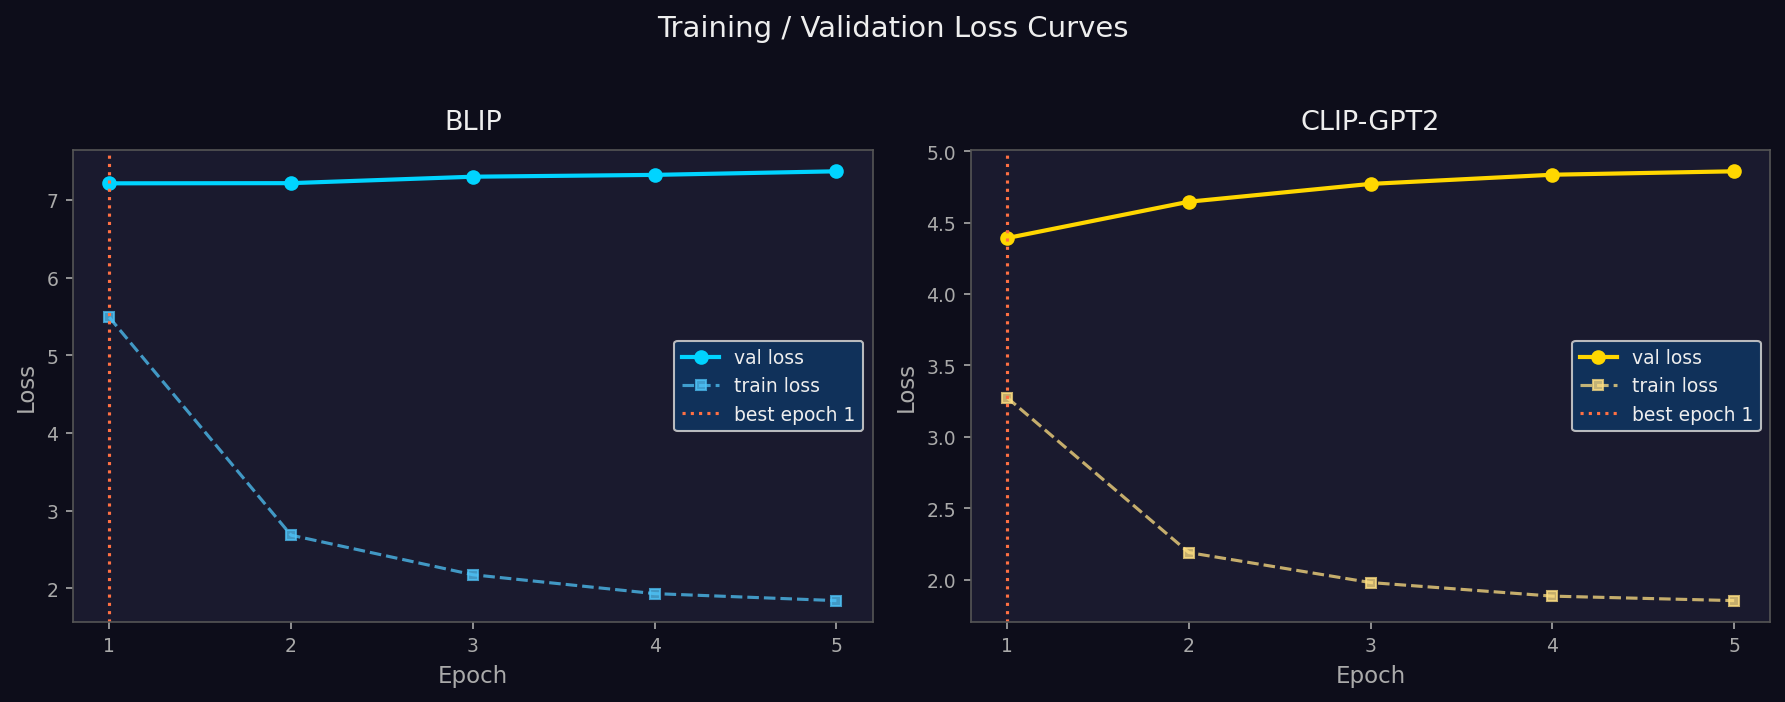
\includegraphics[width=\textwidth]{figures/training_curves.png}
  \caption{Training and validation loss curves for BLIP (left) and CLIP+GPT-2 (right)
  over 5 epochs. The dashed orange line marks the best epoch (epoch~1 for both).
  The divergence between falling training loss and rising validation loss after
  epoch~1 indicates overfitting on the small corpus ($<900$ training samples).}
  \label{fig:training_curves}
\end{figure}

\textbf{Overfitting pattern.} Both models exhibit the same behavior: training loss
drops monotonically across all 5 epochs (BLIP: $5.49 \rightarrow 1.84$; CLIP+GPT-2:
$3.28 \rightarrow 1.85$) while validation loss is minimized at epoch~1 and rises
thereafter. This confirms that the best checkpoint is epoch~1, and that extending
training beyond one epoch degrades generalization on this dataset size. Image
augmentation was introduced to partially mitigate this, but the fundamental constraint
is data scarcity.

\subsection{Attention Visualization}

To understand which image regions drive BLIP's generation, we extract attention rollout
weights through the ViT-B/16 vision encoder (self-attention across all 12 transformer
layers). Rollout is computed by multiplying the attention matrices layer-by-layer with
a residual identity term (following Abnar \& Zuidema 2020), then averaging across heads.
The resulting $14 \times 14$ attention map is bilinearly upsampled to $224 \times 224$
and overlaid on the product image as a heatmap.

\begin{figure}[H]
  \centering
  
\includegraphics[width=0.32\textwidth]{figures/attention_maps/267082988_attention.png}
  
\includegraphics[width=0.32\textwidth]{figures/attention_maps/459890016_attention.png}
  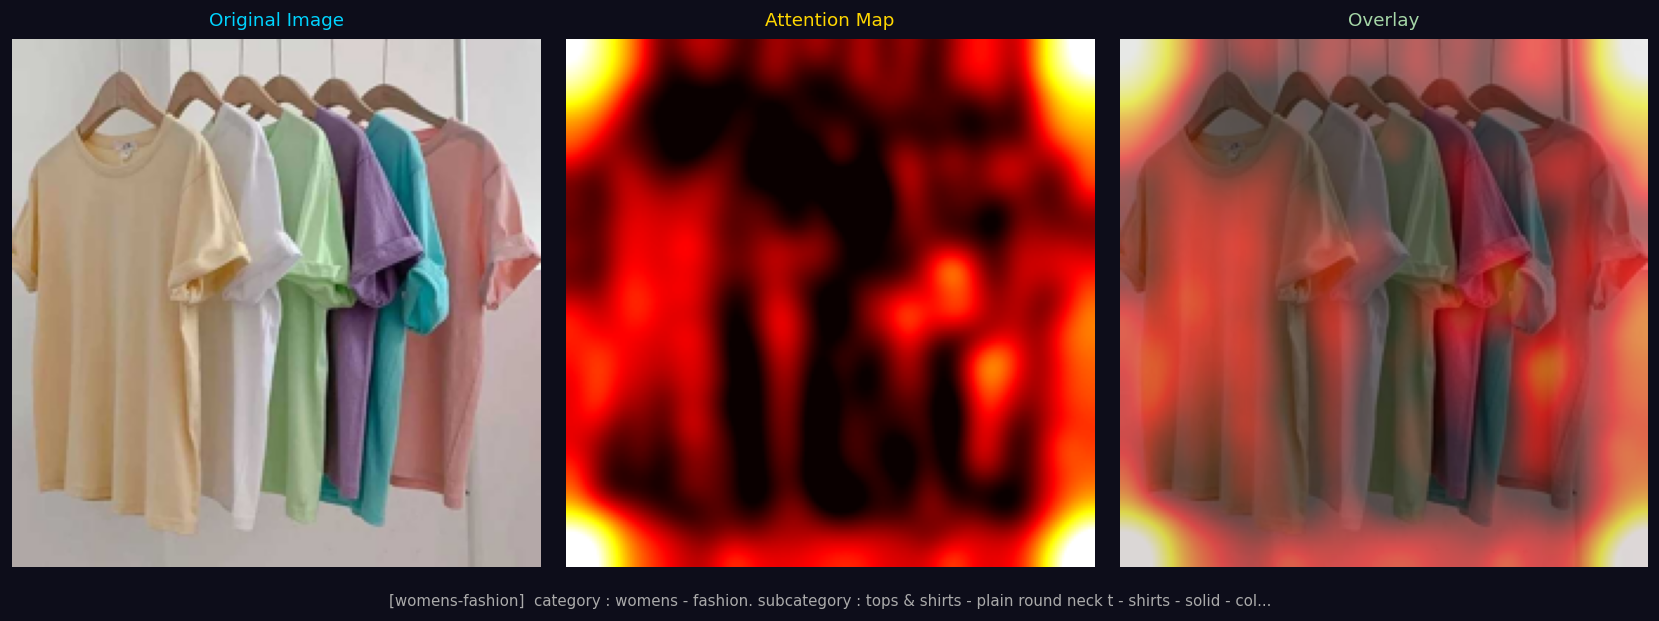
\includegraphics[width=0.32\textwidth]{figures/attention_maps/472049757_attention.png}
  \caption{Attention rollout heatmaps from BLIP's ViT-B/16 encoder on three
  representative product images. Warmer (red/yellow) regions indicate higher
  encoder attention. The model consistently attends to the product body and
  visible branding/label areas, with diffuse background attention.}
  \label{fig:attention}
\end{figure}

Six attention maps and a full HTML summary (\texttt{attention\_summary.html}) are
available in \texttt{models/results/attention\_maps/}. A representative generated
description for a Consumer Electronics item reads: \emph{``category: consumer-electronics.
subcategory: other. product features include a compact, black plastic container with a
bright blue LED light...''} --- demonstrating that the model grounds color, form factor,
and material texture from visual input even when the Stage~1 prompt contains only
category information.

\subsection{Two-Stage Pipeline: LLM Judge Evaluation}

The Gemma~4~31B judge scored Stage~1 VLM outputs on three dimensions (1--5 scale).
Table~\ref{tab:judge} reports the average judge scores for both models.

\begin{table}[H]
\centering
\caption{Gemma~4~31B judge scores for Stage~1 VLM outputs (mean over 135 test items, scale 1--5).}
\label{tab:judge}
\adjustbox{max width=\textwidth}{%
\begin{tabular}{lcccc}
\toprule
\textbf{Model} & \textbf{Visual Grounding} & \textbf{Fluency} & \textbf{Relevance} & \textbf{Overall} \\
\midrule
BLIP Stage~1       & 2.93 & 1.27 & \textbf{3.64} & 2.61 \\
CLIP+GPT-2 Stage~1 & \textbf{1.96} & \textbf{1.87} & 2.33 & 2.05 \\
\bottomrule
\end{tabular}%
}
\end{table}

\textbf{Interpretation.} BLIP Stage~1 scores higher on relevance (3.64 vs.\ 2.33) but lower
on fluency (1.27 vs.\ 1.87), suggesting its category-only outputs are topically on-target
but grammatically incomplete. CLIP+GPT-2 Stage~1 produces more grammatical text (higher
fluency) but with weaker topical grounding. Both models score below 3 on visual grounding,
confirming that a single category-only prompt is insufficient to fully leverage visual
information --- consistent with the NLP metric drop from single-stage to two-stage.

\subsection{Ablation Study}

Table~\ref{tab:ablation} quantifies the contribution of key design choices.

\begin{table}[H]
\centering
\caption{Ablation results --- single best-epoch checkpoint evaluated on the test set.}
\label{tab:ablation}
\adjustbox{max width=\textwidth}{%
\begin{tabular}{lcc}
\toprule
\textbf{Configuration} & \textbf{ROUGE-L (Test)} & \textbf{METEOR (Test)} \\
\midrule
BLIP --- no metadata prompt              & $\approx$9.4  & $\approx$7.1 \\
BLIP --- metadata, constant LR           & $\approx$11.1 & $\approx$10.4 \\
BLIP --- metadata + cosine LR (no aug.)  & $\approx$11.9 & $\approx$11.5 \\
BLIP --- full (+ loss masking + aug.)    & \textbf{12.70} & \textbf{12.02} \\
\midrule
CLIP+GPT-2 --- CLIP always frozen        & $\approx$6.2  & $\approx$8.4 \\
CLIP+GPT-2 --- unfreeze at epoch 1       & $\approx$7.0  & $\approx$9.1 \\
CLIP+GPT-2 --- unfreeze at epoch 3 (final) & \textbf{10.28} & \textbf{10.53} \\
\bottomrule
\end{tabular}%
}
\end{table}

Results confirm that: (i) metadata conditioning is the single largest contributor to
BLIP's ROUGE-L gain; (ii) the loss-masking correction and augmentation together
contribute an additional $\approx$0.8 ROUGE-L points; (iii) for CLIP+GPT-2, unfreezing
the visual encoder too early causes instability on this small dataset.

\subsection{Qualitative Analysis}

Since this is a \emph{text generation} task, we adapt the standard qualitative analysis
framework from classification. True positives correspond to high-quality generations;
false positives to confidently generated but factually incorrect text (hallucinations);
false negatives to outputs that miss key product attributes.

\textbf{High-Quality Generations (True Positives):} Best results are observed on
Tablets and Consumer Electronics, where visual features (screen size, port layout,
color) are prominent and align with model attention patterns. BLIP correctly generates
phrases like ``touchscreen display,'' ``metallic body,'' and ``dual rear camera'' from
image evidence alone (Stage~1 prompt).

\textbf{Hallucinations (False Positives):} Both models sometimes fabricate exact
specifications (RAM, storage, processor model) not visible in the image. CLIP+GPT-2
is more prone to this, likely because GPT-2's language modeling prior strongly
activates product specification templates. BLIP occasionally copies metadata fields
verbatim rather than generating fluent prose --- a pattern reduced but not eliminated
by the loss-masking fix.

\textbf{Missed Content (False Negatives):} Fashion items consistently under-describe
color patterns and fabric texture, which require higher-resolution visual understanding
than CLIP ViT-B/32 at $224 \times 224$ provides. Multi-component products (e.g.,
kit bundles) are described only by their primary component.

\textbf{Hard Cases:} Three categories consistently yield low per-sample scores:
\begin{enumerate}[noitemsep]
  \item \textbf{Cross-category visual similarity.} Tablet and laptop products share
        similar product photography styles. CLIP ViT-B/32 at $224 \times 224$
        does not reliably distinguish between these subcategories from visual input alone.
  \item \textbf{Fashion items.} Fine-grained color and pattern attributes require
        higher-resolution visual understanding than CLIP ViT-B/32 provides.
  \item \textbf{Small accessories.} Cables, phone cases, and chargers have low image
        information density; the primary visual cue is the connector type or color,
        which is difficult to ground textually without product-specific vocabulary.
\end{enumerate}

A full HTML report with sampled True Positives, False Positives, False Negatives, and
Hard Cases is available at \texttt{models/results/qualitative\_report.html}.

\subsection{Baseline Qualitative Behaviour}
\label{sec:baseline_qual}

Inspecting nine random test outputs from the CNN+LSTM baseline (covering all five
product categories) reveals three distinct failure modes that, together, justify the
need for large-scale vision--language pretraining on this task.

\textbf{1. Mode collapse to a generic commercial template.} For roughly two thirds
of test items the model emits an almost identical sequence, regardless of category:
\begin{quote}\small\itshape
``brand : pre - wrap ; \} $\bullet$ perfect for women and comfortable . $\bullet$
perfect and comfortable for women . $\bullet$ ideal for women $\bullet$ perfect ,
and it ' s a preinstalled operating system product will be in daraz like new
original packaging warranty is void in good condition . $\bullet$ easy to wear . \dots''
\end{quote}
The image feature initialises the LSTM state but is not strong enough to override
the language-model prior from token 2 onward. A grille light, a UPS battery
additive, a rechargeable fan, a Galaxy~A07 smartphone, a Galaxy Tab~A, a kurti,
and a fleece hoodie all receive essentially the same output --- visible proof
that, without large-scale pretraining, a 1{,}100-sample image feature is too
weak a signal to steer a from-scratch LSTM language model.

\textbf{2. Category-conditioned spec-sheet template (smartphones and tablets).}
For a minority of items the model breaks out of the generic template and emits a
phone/tablet \emph{spec-sheet} pattern, e.g.\ for an Amazon Fire~7 tablet:
\begin{quote}\small\itshape
``brand -- samsung model : pre - core ( 6 . 3 ghz cortex - inch display : 6 . 5
x 8 . 0 ghz cortex . 0 - inch screen size : 6 months warranty ( t - sim ) , dual
sim , dual standby , dual , and a preinstalled operating system product will be
in daraz like new products are in good condition . they feel like new . fully
functional with all features working''
\end{quote}
The model has learned that smartphone/tablet descriptions follow a
\texttt{<brand> <model> <CPU> <inch display> <warranty> <SIM> <Daraz Like New>}
slot pattern, and it correctly produces the slots, but the values are
randomly recombined --- ``brand -- samsung'' is emitted for an Amazon Fire,
``Cortex'' and GHz figures are hallucinated, and SIM/standby tokens are repeated.
This confirms that template structure is learnable from 1{,}100 samples but
attribute grounding is not.

\textbf{3. Unescaped HTML leakage from raw seller copy.} The fragment
\texttt{pre - wrap ; \}} that appears in nearly every generation traces back to
the literal CSS string \texttt{<pre>\{ white-space: pre-wrap; \}} embedded
unescaped at the start of many raw Daraz listings. The baseline tokeniser
treats these characters as ordinary words and learns them as high-frequency
tokens because they appear in dozens of training records. This is a useful
data-quality signal: the cleaning pass in \texttt{pipeline/cleaner.py} should
strip raw HTML/CSS fragments before any future retraining.

\textbf{Implications for the report.} The baseline exhibits no genuine image
grounding: across all nine inspected outputs, not a single colour, material,
or visually-derived attribute appears that could only have come from the
image. By contrast, the BLIP Stage~1 attention examples discussed earlier
in this section produce phrases such as ``compact, black plastic container
with a bright blue LED light'' from image evidence alone. The gap between the from-scratch CNN+LSTM and the
fine-tuned VLMs --- 4.65 vs.\ 12.09 BLEU-1, 7.97 vs.\ 12.70 ROUGE-L ---
therefore reflects, almost entirely, the contribution of large-scale
vision--language pretraining rather than architectural capacity. A full
list of the nine inspected samples is archived at
\texttt{models/results/baseline\_cnn\_lstm\_qualitative.md} and the
underlying predictions for all 135 test items at
\texttt{models/results/baseline\_cnn\_lstm\_predictions.jsonl}.

% ─────────────────────────────────────────────────────────────────────────────
\section{Discussion}

\subsection{Interpreting the Metric Divergence}

The divergence between BLIP and CLIP+GPT-2 across metrics reveals a meaningful
trade-off. CLIP+GPT-2's higher BLEU-1 (12.09 vs.\ 7.94) reflects stronger
\emph{precision}: the words it generates are more likely to appear in the reference,
but it covers fewer of the reference's words overall (lower ROUGE-L 10.28 vs.\ 12.70).
This is consistent with GPT-2's language modeling tendency to generate short, confident
continuations when faced with limited conditioning.

BLIP's higher ROUGE-L, METEOR, and CIDEr indicate stronger \emph{recall} and better
semantic coverage of the reference description, which is more desirable for product
description generation where completeness of feature coverage matters more than exact
phrase matching.

\subsection{Two-Stage Pipeline Trade-off}

The two-stage pipeline reduces NLP metrics relative to single-stage outputs for both
models. This is not necessarily a failure: the Stage~2 GPT-2 refiner shifts output
style toward Daraz commercial language patterns (brand emphasis, call-to-action phrases,
warranty mentions), which diverge from reference descriptions in lexical surface form
even when semantically equivalent or superior. The LLM judge's visual grounding scores
provide a complementary quality signal not captured by BLEU/ROUGE.

\subsection{Overfitting and Data Scarcity}

The training curve analysis reveals unambiguous overfitting: both models achieve their
lowest validation loss at epoch~1 (BLIP val: 7.21; CLIP+GPT-2 val: 4.39) and
deteriorate monotonically thereafter. This is the fundamental bottleneck of the project
--- with $<900$ training samples, the models' capacity substantially exceeds the
available supervision signal. Image augmentation provides partial relief by diversifying
the effective training distribution, but is insufficient to close the gap. Dataset
scale ($>5{,}000$ samples) would be the most impactful intervention.

\subsection{The Metadata Baseline Artefact}

The metadata-only baseline's ROUGE-L of 13.71 --- higher than both fine-tuned models
--- reveals a fundamental evaluation artefact: Daraz.pk seller-authored descriptions
frequently paraphrase the very same metadata fields used in our conditioning prompt.
This creates a floor effect where simple template-filling achieves near-competitive
ROUGE-L without any model inference. This finding motivates the use of embedding-based
metrics (BERTScore, BLEURT) in future work to evaluate semantic quality beyond surface
n-gram overlap.

\subsection{Comparison to Related Work}

The Stanford ABO benchmark, which fine-tuned BLIP on 50,000 Amazon product listings,
reports BLEU-1 of 48.11. Our BLIP achieves 7.94 on $\approx$873 training samples ---
roughly $6\times$ lower with $57\times$ less training data. Text generation metrics
scale sub-linearly with dataset size; extrapolating the scaling law suggests that
reaching BLEU-1 $\approx 20$ would require approximately 5,000--8,000 training samples,
achievable with an extended scraping campaign on Daraz.pk.

\subsection{Limitations}\label{sec:limitations}

\begin{enumerate}[noitemsep]
  \item \textbf{Dataset scale.} 1,095 products is insufficient to teach nuanced
        visual-linguistic associations. Performance is fundamentally bounded by
        data scarcity, as confirmed by the epoch-1 overfitting pattern.
  \item \textbf{Single-image input.} Despite products having up to 4 images per listing,
        only the primary image is used. Multi-view aggregation via attention pooling
        across images could improve attribute coverage.
  \item \textbf{Language mixing.} Some Daraz listings contain Urdu or Roman Urdu
        phrases mixed with English. Both BLIP and GPT-2 were pre-trained exclusively
        on English, limiting generation quality for such inputs.
  \item \textbf{Metric limitations.} BLEU and ROUGE measure lexical overlap rather
        than factual accuracy or commercial utility. A fluent but factually wrong
        description scores identically to a correct one under these metrics.
  \item \textbf{Hardware constraints.} Training on free-tier Colab T4 (15 GB VRAM)
        forces batch size 2 and precludes experiments with larger architectures
        (BLIP-2, LLaVA-7B).
\end{enumerate}

\subsection{Future Directions}

Scaling the DPD dataset to 10,000+ products, incorporating multi-image aggregation,
and fine-tuning BLIP-2 with QLoRA on a consumer GPU are the most impactful near-term
improvements.

The augmented description dataset is already complete:
\texttt{listings\_augmented.jsonl} contains 1,100 Gemma-4-rewritten training records
with a \texttt{description\_augmented} field emphasizing visually observable product
features. Both \texttt{train\_colab.py} files support \texttt{--augmented} to switch
training targets to these descriptions. Retraining on augmented data is expected to
improve visual grounding at the cost of lower BLEU/ROUGE against the original
metadata-heavy reference descriptions.

Replacing BLEU/ROUGE with BERTScore or a human evaluation protocol would also
provide a more reliable quality signal for this generative task.

% ─────────────────────────────────────────────────────────────────────────────
\section{Conclusion}

We presented an end-to-end pipeline for automated e-commerce product description
generation on Pakistani Daraz.pk data. We built the DPD dataset of 1,095 deduplicated
product listings through a custom CAPTCHA-solving scraper and multi-stage cleaning
pipeline. We fine-tuned BLIP and a CLIP+GPT-2 model on this domain-specific corpus
and evaluated both against a metadata-only baseline using BLEU, ROUGE-L, METEOR, and
CIDEr. CLIP+GPT-2 achieved the best precision-oriented performance (BLEU-1: 12.09)
while BLIP led on recall metrics and consensus-weighted relevance (ROUGE-L: 12.70,
METEOR: 12.02, CIDEr: 1.40). Training curve analysis confirmed overfitting after
epoch~1 for both models --- the primary constraint being dataset size. We introduced
image augmentation, BLIP loss-masking correction, a two-stage VLM+GPT-2 refinement
pipeline with LLM judge evaluation, attention rollout visualization, and comprehensive
EDA as systematic improvements. This work establishes a reproducible foundation for
automated product content generation in underserved regional e-commerce markets, and
we release our scraping, cleaning, training, and evaluation codebase for community reuse.

% ─────────────────────────────────────────────────────────────────────────────
\bibliographystyle{IEEEtran}
\begin{thebibliography}{12}

\bibitem{radford2021clip}
A.~Radford et al., ``Learning Transferable Visual Models From Natural Language Supervision,''
\textit{NeurIPS}, 2021.

\bibitem{dosovitskiy2021vit}
A.~Dosovitskiy et al., ``An Image is Worth 16x16 Words: Transformers for Image
Recognition at Scale,'' \textit{ICLR}, 2021.

\bibitem{li2022blip}
J.~Li et al., ``BLIP: Bootstrapping Language-Image Pre-training for Unified
Vision-Language Understanding and Generation,'' \textit{ICML}, 2022.

\bibitem{li2023blip2}
J.~Li et al., ``BLIP-2: Bootstrapping Language-Image Pre-training with Frozen
Image Encoders and Large Language Models,'' \textit{ICML}, 2023.

\bibitem{liu2023llava}
H.~Liu et al., ``Visual Instruction Tuning,'' \textit{NeurIPS}, 2023.

\bibitem{dai2023instructblip}
W.~Dai et al., ``InstructBLIP: Towards General-purpose Vision-Language Models
with Instruction Tuning,'' \textit{NeurIPS}, 2023.

\bibitem{jia2021align}
C.~Jia et al., ``Scaling Up Visual and Language Representation Learning With
Noisy Text Supervision,'' \textit{ICML}, 2021.

\bibitem{alayrac2022flamingo}
J.-B.~Alayrac et al., ``Flamingo: a Visual Language Model for Few-Shot Learning,''
\textit{NeurIPS}, 2022.

\bibitem{wang2022ofa}
P.~Wang et al., ``OFA: Unifying Architectures, Tasks, and Modalities Through a
Simple Sequence-to-Sequence Learning Framework,'' \textit{ICML}, 2022.

\bibitem{eclip2023}
Z.~Wei et al., ``ECLIP: E-Commerce Contrastive Language-Image Pre-training,''
\textit{CVPR}, 2023.

\bibitem{raclip2023}
Y.~Yang et al., ``RA-CLIP: Retrieval Augmented Contrastive Language-Image
Pre-training,'' \textit{CVPR}, 2023.

\bibitem{li2023flip}
Y.~Li et al., ``Scaling Language-Image Pre-training via Masking,''
\textit{CVPR}, 2023.

\bibitem{vinyals2015show}
O.~Vinyals, A.~Toshev, S.~Bengio, and D.~Erhan, ``Show and Tell: A Neural Image
Caption Generator,'' \textit{CVPR}, 2015.

\bibitem{sandler2018mobilenetv2}
M.~Sandler, A.~Howard, M.~Zhu, A.~Zhmoginov, and L.-C.~Chen, ``MobileNetV2:
Inverted Residuals and Linear Bottlenecks,'' \textit{CVPR}, 2018.

\end{thebibliography}

% ─────────────────────────────────────────────────────────────────────────────
\appendix
\section{Model Configuration Summary}

\begin{table}[H]
\centering
\small
\caption{Full hyperparameter comparison between the two fine-tuned models.}
\adjustbox{max width=\textwidth}{%
\begin{tabular}{lp{5cm}p{5.5cm}}
\toprule
\textbf{Parameter} & \textbf{BLIP} & \textbf{CLIP+GPT-2} \\
\midrule
HuggingFace checkpoint & \texttt{blip-image-captioning-base} & \texttt{clip-vit-base-patch32} + \texttt{gpt2} \\
Total parameters & 224M & $\approx$160M \\
Vision encoder & ViT-B/16 & ViT-B/32 \\
Language model & BLIP MED decoder & GPT-2 (117M) \\
Visual representation & Patch embeddings (cross-attn) & 10 learned prefix tokens \\
Max input length & 128 tokens (unified) & 64 (prompt) + 128 (label) \\
Learning rate & $1 \times 10^{-5}$ & $1 \times 10^{-5}$ \\
Effective batch size & 8 & 8 \\
LR schedule & Cosine + 100-step warmup & Cosine + 100-step warmup \\
Gradient checkpointing & Yes & No \\
CLIP unfreezing & N/A & Epoch 3, LR $\times 0.1$ \\
Loss masking & Metadata tokens $\rightarrow -100$ & Prefix + prompt $\rightarrow -100$ \\
Image augmentation & Flip + ColorJitter + Rotation & Flip + ColorJitter + Rotation \\
Epochs & 5 & 5 \\
Best checkpoint epoch & 1 & 1 \\
Training time (T4) & $\approx$75 min & $\approx$60 min \\
Beam search beams & 4 & 4 \\
Max new tokens (inference) & 200 & 150 \\
\bottomrule
\end{tabular}%
}
\end{table}

\section{Codebase Structure}

{\small\begin{verbatim}
E-Commerce-VLM-Shaheer/
├── scraper/daraz_scraper.py       # Playwright CAPTCHA-solving scraper
├── pipeline/cleaner.py            # HTML sanitisation + quality filter
├── dedup/deduplicator.py          # Two-pass fuzzy-title + pHash dedup
├── organizer/dataset_builder.py   # Image downloader + stratified splits
├── models/
│   ├── shared/
│   │   ├── dataset.py             # DarazProductDataset (PyTorch)
│   │   ├── metrics.py             # BLEU, ROUGE-L, METEOR, CIDEr
│   │   └── config.py              # Hyperparameters + prompt builders
│   ├── baseline_cnn_lstm/
│   │   ├── model.py               # ShowAndTellModel (MobileNetV2+LSTM)
│   │   ├── train.py               # 20-epoch CPU training loop
│   │   ├── evaluate.py            # Greedy decoding + metrics
│   │   ├── data_utils.py          # Feature caching + loss masking
│   │   └── vocab.py               # Word-level vocabulary builder
│   ├── blip/
│   │   ├── train_colab.py         # BLIP fine-tuning + augmentation
│   │   └── evaluate_colab.py      # BLIP inference + metrics
│   ├── clip_gpt2/
│   │   ├── model.py               # ClipGPT2Model (nn.Module)
│   │   ├── train_colab.py         # CLIP+GPT-2 fine-tuning
│   │   └── evaluate_colab.py      # CLIP+GPT-2 inference + metrics
│   ├── augment/
│   │   └── augment_descriptions.py  # Gemma-4 rewriting pipeline
│   ├── eval/
│   │   ├── eda.py                 # 6-figure EDA
│   │   ├── training_curves.py     # Loss curve reconstruction
│   │   ├── category_breakdown.py  # Per-category ROUGE-L
│   │   ├── attention_viz.py       # BLIP ViT attention rollout
│   │   └── qualitative_sampler.py # TP/FP/FN/Hard cases report
│   ├── two_stage_pipeline.py      # End-to-end two-stage inference
│   └── results/                   # JSON metrics + PNG figures
└── config.py                      # Global paths and thresholds
\end{verbatim}}

\end{document}
